\documentclass[parskip=full,11pt]{scrartcl}
%\usepackage{pdfpages}
\usepackage[utf8]{inputenc}
\usepackage[T1]{fontenc}
\usepackage[german]{babel}
\usepackage[yyyymmdd]{datetime} 
\usepackage{hyperref}
\usepackage[toc, nonumberlist]{glossaries}
\usepackage{csquotes}
\usepackage{graphicx}
\hypersetup{
 		pdftitle={Entwurf},
 		bookmarks=true,
 }
\usepackage{fancyhdr}%<-------------to control headers and footers
\usepackage[a4paper,margin=1in,footskip=.25in]{geometry}
\fancyhf{}
\fancyfoot[C]{\thepage} %<----to get page number below text
\pagestyle{fancy} %<-------the page style itself
 
\title{Entwurf}
\subtitle{Autorisierungsmanagement für eine virtuelle Forschungsumgebung für Geodaten}
\author{Alex\\Anastasia\\Atanas\\Dannie\\ Houra\\Sonya\\}
\date{11.01.18}
 % define custom lists
\usepackage{enumitem}



\usepackage{linegoal,listings}
\newsavebox{\mylisting}
\makeatletter
\newcommand{\lstInline}[2][,]{%
	\begingroup%
	\lstset{#1}% Set any keys locally
	\begin{lrbox}{\mylisting}\lstinline!#2!\end{lrbox}% Store listing in \mylisting
	\setlength{\@tempdima}{\linegoal}% Space left on line.
	\ifdim\wd\mylisting>\@tempdima\hfill\\\fi% Insert line break
	\lstinline!#2!% Reset listing
	\endgroup%
}
\makeatother
\setlength{\parindent}{0pt}% Just for this example

\lstset{basicstyle=\footnotesize\ttfamily,breaklines=true}
\lstset{framextopmargin=50pt,frame=bottomline,showstringspaces=false,upquote=true}


\RedeclareSectionCommand[style=section,indent=0pt,font=\usekomafont{partnumber}]{part}
\renewcommand*{\partformat}{\thepart\enskip}

\RedeclareSectionCommand[beforeskip=0pt ,afterskip=0pt]{subparagraph}



\newcommand{\class}[1]{\subsubsection*{\lstinline[basicstyle=\ttfamily\large]{#1}}}

% command for an attribute
\newcommand{\atr}[4]{\lstinline{[#3]} \textbf{\lstinline{#1 : #2}} \newline #4}

% command for a method
\newcommand{\mtd}[5]{\lstinline{[#4]} \textbf{\lstinline{#1(#3) : #2}} \newline #5}

% command for a constructor
\newcommand{\ctr}[4]{\lstinline{[#3]} \textbf{\lstinline{#1(#2)}} \newline #4}
%command for formating an inline source code
\newcommand{\inlinecode}[1]{\lstInline[breaklines=true]{#1}}

% make the bullet symbol in lists a circle for level 2
\renewcommand{\labelitemii}{$\circ$}




 
\begin{document}
 
 \begin{titlepage}
 	
 	\begin{center}
 	
\includegraphics[width=0.5\linewidth]{res/KITLogo.png}\\
 	\vspace{2cm}
 	{\scshape\LARGE\bfseries Entwurf \par}
 	\vspace{0.5cm}
 	{\scshape\Large Praxis der Softwareentwicklung\\}
 	\vspace{1cm}
 	{\scshape\Large Wintersemester 17/18\\}
 	\vspace{2cm}
 	{\huge\bfseries Autorisierungsmanagement für eine virtuelle Forschungsumgebung für Geodaten\par}
 	\vspace{2cm}
 	\vfill
 	{\bfseries {\Large Autoren}:\par}
 	{\Large Bachvarov, Aleksandar }\\
 	{\Large Dimitrov, Atanas }\\
 	{\Large Mortazavi Moshkenan, Houraalsadat }\\
 	{\Large Sakly, Khalil }\\
 	{\Large Slobodyanik, Anastasia }\\
 	{\Large Voneva, Sonya}\\
 	\vfill
 	{\large 11.01.18 \par}
 	\end{center}
 \end{titlepage}
 
 \tableofcontents
 
 \newpage
 \section{Einleitung}
 
 \subsection{Änderung zum Pflichtenheft}

 %Wunschkriterien, die wir implementieren moechten
 
 \section{Architektur}
 
 \subsection{Model View Template (MVT)} 
\begin{figure}[h]
 \centering
 Beim Design des Autorisierungsmanagement Web-Portal wird schnell deutlich, dass eine strikte Trennung
zwischen Datenbank, Applikationslogik (Code) und Benutzeroberfläche (view) von Vorteil ist. Das Model-View-Template-Prinzip (MVT) realisiert diese Trennung und wird in der Webanwendung eingesetzt.
  	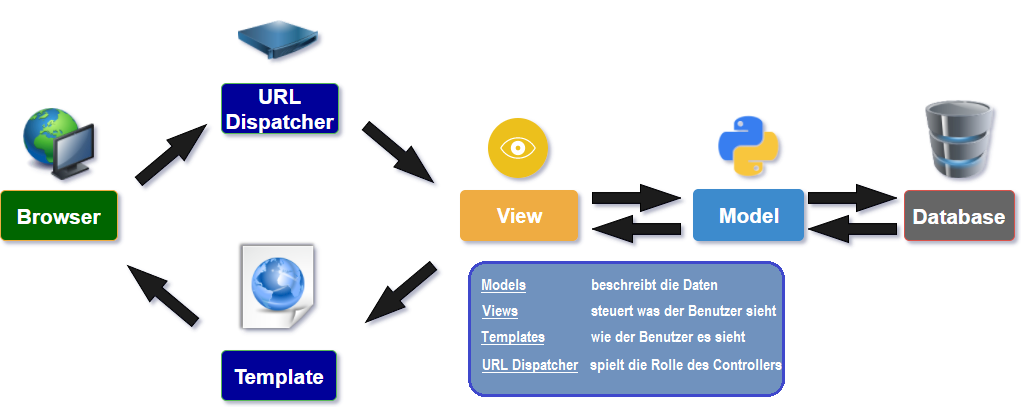
\includegraphics[width=18cm, height=12cm]{res/MVT diagramm.png}\\
  	    \caption{MVT Architektur}

  	 \label{fig:abb1}

 	\vspace{2cm}
 	1-Der URL-Dispatcher (urls.py) ordnet die angeforderte URL einer View-Funktion zu und ruft sie auf.\\
 	2-Die View-Funktion (views.py) führt die angeforderte Aktion aus, bei der normalerweise in die Datenbank gelesen oder geschrieben wird. es kann auch andere Aufgaben beinhalten.\\
 	3-Das Model (models.py) definiert die Daten in Python und interagiert damit. Dies ist normalerweise in einer relationalen Datenbank (SQLite) enthalten.\\
 	4-Nach der Ausführung der angeforderten Aufgaben gibt die View ein HTTP-Antwortobjekt an den Webbrowser zurück, normalerweise nach dem Übergeben der Daten durch ein Template.\\
 	5-Template gibt normalerweise HTML-Seiten zurück. Die Django-Template-sprache bietet HTML-Autoren eine einfach zu erlernende Syntax und bietet gleichzeitig die gesamte für die Präsentationslogik erforderliche Leistung. \\


 	\end{figure}


 \subsection{Paketstruktur}%oder Paketen?
 
 \subsection{Entwurfsmuster}
 
 
 \section{Datenhaltung}
 %\subsection{Datenbank}
 %\subsection{Log Datei}
 
 
 \section{Paketenübersicht}
 
 
 \section{Klassenübersicht}
 
  \paragraph*{Klasse Owner}
 \class{Owner extends User}
 bla bla
 
 \subparagraph*{Konstruktoren} % skip this if there are no constructors
\begin{itemize}
	\item \ctr{User}{a:String}{public}{
	bla
	}
\end{itemize}
\paragraph*{Attribute} % skip this if there are no attribute
\begin{itemize}
	\item \atr{name}{String}{private}{
	bla 
	}
\end{itemize}
\subparagraph*{Methoden}  % skip this if there are no methods
\begin{itemize}
	\item \mtd{foo}{String}{a:String}{public}{
	bla  \inlinecode{USER_ID}
	}
\end{itemize}
 
 \section{Sonstige Diagrammen}
 
 
 
 \newpage
	
 \end{document}
 \grid
